\documentclass[12pt,fleqn]{article}\usepackage{../../common}
\begin{document}
Frekans Analizi, Periyodik Sinyaller

Bir periyodik sinyali nasil analiz ederiz? Kendimiz bir sinyal olusturmak
istesek, bunu nasil yapacagimizi dusunelim; $\sin$ ya da $\cos$
matematiksel fonksiyonlarinin bir periyotu vardir, $0,2\pi$ arasindaki
degerleri $2\pi,4\pi$ arasinda tekrar eder, boyle devam eder. Tabii
periyodik sinyallerin ek ozellikleri olabilir, mesela $\cos$ sifir
noktasinda 1 degerine sahiptir, fakat elimizdeki zaman serisi saga ya da
sola ``kaymis'' olabilir, yani sifir noktasinda deger 1 degildir. Ayrica
-1,+1 arasinda gidip gelmek yerine mesela -10,+10 arasinda gidip
gelinebilir. Bir diger ozellik $0,2\pi$ arasinda tek bir periyot yerine
birden fazla periyot olabilmesi (frekans). 

Frekans ile baslayalim, 

\begin{minted}[fontsize=\footnotesize]{python}
x = np.linspace(0,10,100)
plt.plot(x, np.cos(x))
plt.xlim(0,10)
plt.savefig('tser_freq_01.png')
\end{minted}

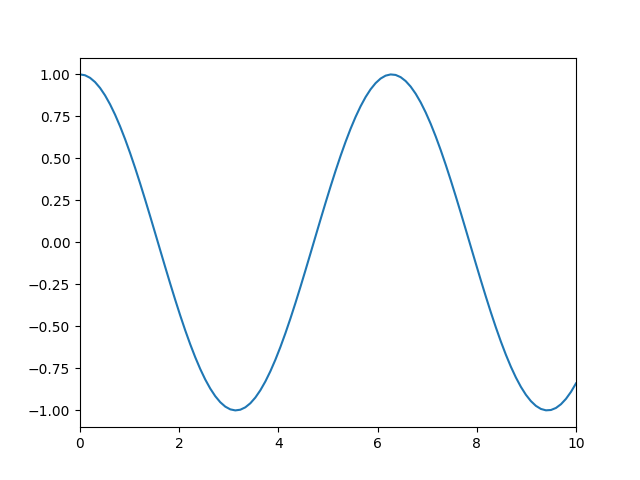
\includegraphics[height=6cm]{tser_freq_01.png}

\begin{minted}[fontsize=\footnotesize]{python}
x = np.linspace(0,10,100)
plt.plot(x, np.cos(x))
plt.axvline(0,lw='1',ls='dashed',color='r')
plt.axvline(np.pi,lw='1',ls='dashed',color='r')
plt.axvline(2*np.pi,lw='1',ls='dashed',color='r')
plt.axvline(3*np.pi,lw='1',ls='dashed',color='r')
plt.xlim(0,10)
plt.savefig('tser_freq_02.png')
\end{minted}

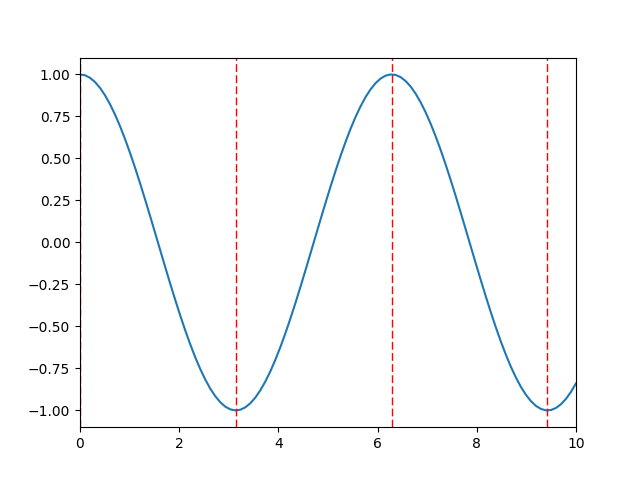
\includegraphics[height=6cm]{tser_freq_02.png}

\begin{minted}[fontsize=\footnotesize]{python}
plt.plot(x, np.cos(2*x))
plt.axvline(0,lw='1',ls='dashed',color='r')
plt.axvline(np.pi,lw='1',ls='dashed',color='r')
plt.axvline(2*np.pi,lw='1',ls='dashed',color='r')
plt.axvline(3*np.pi,lw='1',ls='dashed',color='r')
plt.xlim(0,10)
plt.savefig('tser_freq_03.png')
\end{minted}

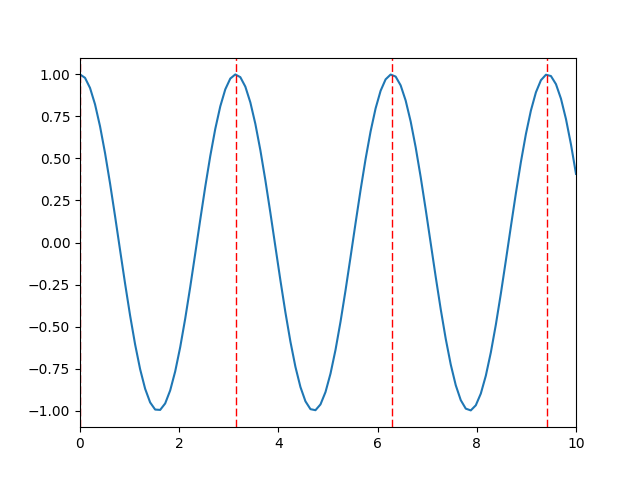
\includegraphics[height=6cm]{tser_freq_03.png}

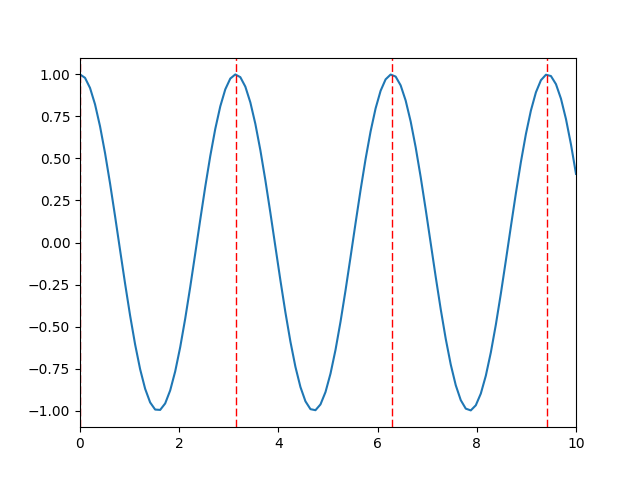
\includegraphics[height=4cm]{tser_freq_03.png}

















\end{document}






















